% Provenance (never printed): see sources/outline_sources.md (Year 2: partial melting of the
% mantle; solidus and geotherm; decompression, hydration and heating; degree of melting;
% binary and ternary phase diagrams applied to rocks).
% Curves from figdata/bachelor-2/melting.py (Bowen 1915 diopside-anorthite, Bowen and
% Andersen 1914 forsterite-silica, Katz et al. 2003 melting of peridotite); exercise and
% problem values in the Book 4 scratch calculator calc/ch07.py.
\chapter{Pelelehan Mantel}\label{ch:b2:mantle-melting}

Mantel itu padat. Gelombang geser seismik menembusnya dari atas sampai bawah, dan
\omterm{def:b2:mantle-melting:peridotites}{peridotit} yang terangkat dari sana adalah batuan kristalin. Namun, di sepanjang punggungan samudra
saja, mantel menghasilkan sekitar dua puluh kilometer kubik kerak samudra baru setiap tahun,
dan setiap meter kubiknya dibuat dari lelehan. Paradoks itu lenyap begitu kita tahu
bahwa mantel tidak meleleh karena dipanaskan: mantel meleleh karena
tekanan yang menindihnya turun, atau karena air ditambahkan ke dalamnya. Di bawah punggungan,
mantel naik, tekanannya turun lebih cepat daripada suhunya, dan mantel itu melintasi
kurva pelelehannya; di atas slab yang tenggelam, air yang dilepaskan slab menurunkan kurva itu
di bawah baji mantel. Dalam kedua kasus hanya sebagian kecil batuan yang
meleleh, dan bagian itu, setelah terpisah dari residunya, menjadi basal
dasar samudra dan busur vulkanik. Bab ini mula-mula memerikan batuan
mantel dan diagram fase yang menunjukkan bagaimana batuan semacam itu meleleh, lalu mengikuti
mantel yang naik di bawah punggungan sampai ke tebal kerak yang dibuatnya.
% ledger: white:crust (Book 3), data:pb2002 (Book 3), katz03:solidus

\begin{recall}
\textbf{Dari volume Tahun 2 buku kimia}: diagram fase biner,
solidus dan likuidus, titik eutektik, pelelehan kongruen, larutan padat,
dan aturan tuas, yang menyatakan bahwa proporsi dua fase yang berdampingan
berbanding terbalik dengan jaraknya dari komposisi total.
\textbf{Dari buku-buku fisika}: kalor jenis, kalor laten, entropi,
dan hukum kedua, yang menyatakan bahwa proses adiabatik reversibel mempertahankan entropi.
\textbf{Dari volume Tahun 1}: mineral-mineral utama pembentuk batuan, olivin,
piroksen, garnet, dan spinel, larutan padatnya, dan bilangan Mg;
adiabat mantel, $\mathrm dT/\mathrm dz = \alpha gT/c_p$; kerak samudra, yang tebalnya
\qty[uncertainty-mode=separate]{7.1 \pm 0.8}{km} jauh dari titik panas dan
sekitar \qty{20}{km} di atas inti plume; slab yang menunjam dan air yang
dibawanya. \textbf{Dari \cref{ch:b2:elements-in-the-earth}}: \omterm{def:b2:elements-in-the-earth:morb-oib}{basal punggungan tengah samudra}
(MORB), koefisien partisi, dan \omterm{def:b2:elements-in-the-earth:partition}{unsur inkompatibel}.
\end{recall}

\section{Batuan mantel}\label{sec:b2:mantle-melting:rock}

Batuan mantel sampai ke permukaan sebagai fragmen yang terbawa naik oleh \omterm{def:b2:magma-emplacement:magma}{magma},
yaitu xenolit, dan sebagai bagian dasar irisan litosfer samudra yang terdorong ke atas
benua, yaitu ofiolit. Hampir semuanya berupa \omterm{def:b2:mantle-melting:peridotites}{peridotit}.
% ledger: geo:peridotite (Book 2), tulane:ocean-basins (Book 2)

\begin{definition}[Peridotit dan jenis-jenisnya]\label{def:b2:mantle-melting:peridotites}
Yang disebut \emph{peridotit}\index{peridotit} adalah batuan ultramafik berbutir kasar
yang mengandung lebih dari \qty{40}{\percent} olivin, sisanya berupa piroksen dan
sedikit mineral beraluminium (spinel atau garnet). Yang disebut
\emph{dunit}\index{dunit} mengandung lebih dari \qty{90}{\percent} olivin. Di bawah
batas itu, \emph{lherzolit}\index{lherzolit} mengandung ortopiroksen dan
klinopiroksen sekaligus; \emph{harzburgit}\index{harzburgit} mengandung ortopiroksen tetapi
hampir tidak mengandung klinopiroksen; wehrlit mengandung klinopiroksen tetapi hampir tidak mengandung
ortopiroksen. Batuan dengan olivin kurang dari \qty{40}{\percent} disebut piroksenit.
\end{definition}
% ledger: bgs:ultramafic

Klasifikasi ini dibaca pada sebuah segitiga yang sudut-sudutnya olivin,
ortopiroksen, dan klinopiroksen (gambar di bawah): setiap titik mewakili satu batuan,
dan jaraknya dari ketiga sisi memberikan proporsi ketiga
mineral itu. Komposisi model mantel atas terkuras yang meleleh di bawah
punggungan terdiri atas \qty{57}{\percent} olivin,
\qty{28}{\percent} ortopiroksen, \qty{13}{\percent} klinopiroksen, dan
\qty{2}{\percent} spinel: sebuah \omterm{def:b2:mantle-melting:peridotites}{lherzolit}.
% ledger: liang21:dmm-mode

\begin{omfigure}
\centering
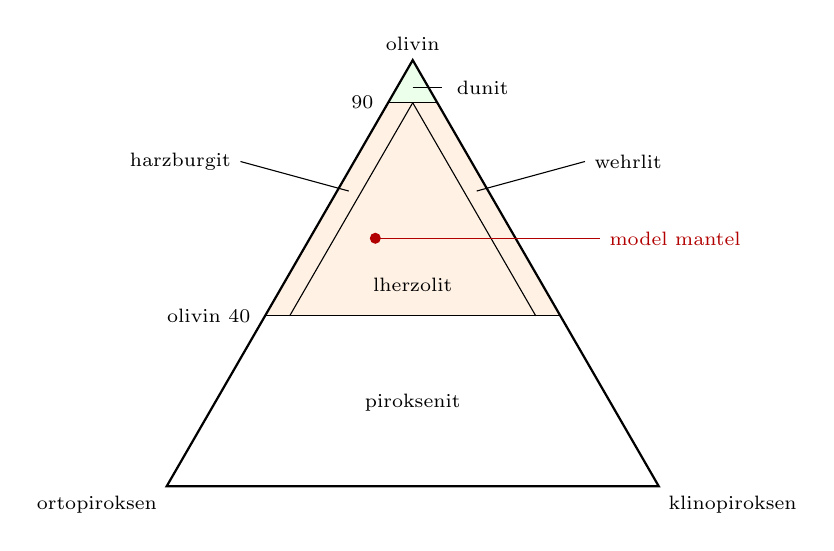
\begin{tikzpicture}[x=1.25cm, y=1.25cm, font=\scriptsize]
\coordinate (O) at (2.5,4.330); \coordinate (P) at (0,0); \coordinate (C) at (5,0);
\fill[green!8] (2.25,3.897) -- (2.75,3.897) -- (O) -- cycle;
\fill[orange!10] (1,1.732) -- (2.25,3.897) -- (2.75,3.897) -- (4,1.732) -- cycle;
\draw[thick] (O) -- (P) -- (C) -- cycle;
\draw (2.25,3.897) -- (2.75,3.897);
\draw (1,1.732) -- (4,1.732);
\draw (2.5,3.897) -- (1.25,1.732);
\draw (2.5,3.897) -- (3.75,1.732);
\node[anchor=south] at (O) {olivin};
\node[anchor=north east] at (P) {ortopiroksen};
\node[anchor=north west] at (C) {klinopiroksen};
\node[anchor=west] at (2.85,4.05) {dunit};
\draw (2.5,4.05) -- (2.8,4.05);
\node at (2.5,2.05) {lherzolit};
\draw (1.85,3.0) -- (0.75,3.3) node[anchor=east] {harzburgit};
\draw (3.15,3.0) -- (4.25,3.3) node[anchor=west] {wehrlit};
\node at (2.5,0.85) {piroksenit};
\node[anchor=east] at (0.95,1.732) {olivin \qty{40}{\percent}};
\node[anchor=east] at (2.2,3.897) {\qty{90}{\percent}};
\fill[red!70!black] (2.12,2.52) circle (2pt);
\draw[red!70!black] (2.12,2.52) -- (4.4,2.52) node[anchor=west] {model mantel};
\end{tikzpicture}
\par\smallskip{\small Klasifikasi \omterm{def:b2:mantle-melting:peridotites}{peridotit} dan piroksenit berdasarkan
proporsi olivin, ortopiroksen, dan klinopiroksennya (menurut skema British
Geological Survey). Jalur sempit di sepanjang kedua sisi atas memuat
batuan yang hampir tidak mengandung klinopiroksen (\omterm{def:b2:mantle-melting:peridotites}{harzburgit}) atau ortopiroksen (wehrlit).
Titik merah adalah model mantel atas di bawah punggungan (57, 28, dan
\qty{13}{\percent}, dinormalkan ulang tanpa \qty{2}{\percent} spinelnya).}
\end{omfigure}
% ledger: bgs:ultramafic, liang21:dmm-mode

Ketiga \omterm{def:b2:mantle-melting:peridotites}{peridotit} itu bukan tiga jenis batuan yang berdiri sendiri: ketiganya adalah tahap-tahap
satu proses. Klinopiroksen dan mineral beraluminium habis lebih dahulu ketika
\omterm{def:b2:mantle-melting:peridotites}{peridotit} meleleh (\cref{sec:b2:mantle-melting:decompression}), sehingga \omterm{def:b2:mantle-melting:peridotites}{lherzolit}
yang telah kehilangan lelehan menjadi lebih miskin akan keduanya; setelah pelelehan yang cukup, batuan itu menjadi
\omterm{def:b2:mantle-melting:peridotites}{harzburgit}, dan batuan yang telah kehilangan hampir seluruh piroksennya menjadi \omterm{def:b2:mantle-melting:peridotites}{dunit}.
% ledger: katz03:melting

\begin{definition}[Mantel subur dan mantel residu]\label{def:b2:mantle-melting:fertility}
Yang disebut \emph{mantel subur}\index{mantel subur} adalah \omterm{def:b2:mantle-melting:peridotites}{peridotit}, biasanya
\omterm{def:b2:mantle-melting:peridotites}{lherzolit}, yang masih mengandung klinopiroksen dan mineral beraluminium yang menjadi bahan
pembuat basal. Yang disebut \emph{mantel residu}\index{mantel residu} adalah
\omterm{def:b2:mantle-melting:peridotites}{peridotit} yang tertinggal setelah lelehan diekstraksi darinya: lebih miskin akan
klinopiroksen, aluminium, kalsium, dan \omterm{def:b2:elements-in-the-earth:partition}{unsur inkompatibel}, lebih kaya akan
olivin, dan dengan bilangan Mg yang lebih tinggi.
\end{definition}

\omterm{def:b2:isotope-geochemistry:reservoirs}{Mantel terkuras} isotopik pada \cref{ch:b2:isotope-geochemistry} adalah sebuah reservoir,
yang didefinisikan oleh rasio-rasionya; \omterm{def:b2:mantle-melting:fertility}{mantel residu} adalah batuan, yang didefinisikan oleh apa yang telah hilang darinya.
Keduanya berkaitan, karena \omterm{def:b2:isotope-geochemistry:reservoirs}{mantel terkuras} itu terkuras justru karena lelehan
diekstraksi darinya sejak lama, tetapi yang satu dibaca dengan spektrometer massa dan yang lain
di bawah mikroskop.

\section{Diagram fase batuan}\label{sec:b2:mantle-melting:diagrams}

Batuan adalah campuran mineral, dan batuan meleleh dalam suatu rentang suhu, bukan pada
satu titik. Diagram yang memerikan hal ini mula-mula diukur pada campuran
mineral sintetis murni, dengan menahan sedikit cuplikan pada suhu yang diketahui sampai
mencapai kesetimbangan, mendinginkannya secara mendadak (quenching), lalu mencari di bawah mikroskop kaca,
yang semula cair, dan kristal.

\subsection*{Eutektik biner: diopsid dan anortit}

Basal pada dasarnya terdiri atas plagioklas kalsik dan klinopiroksen, dan
Bowen memilih anortit dan diopsid murni sebagai model paling sederhananya. Bila dicampur dan dipanaskan,
keduanya membentuk sistem eutektik
biasa (gambar di bawah): diopsid meleleh pada \qty{1391.5}{\celsius} dan anortit
pada \qty{1550}{\celsius}, tetapi campuran \qty{58}{\percent} diopsid dan
\qty{42}{\percent} anortit menurut massa meleleh seluruhnya pada \qty{1270}{\celsius}.
% ledger: bowen15:di-an

\begin{omfigure}
\centering
\begin{tikzpicture}
\begin{axis}[omrecord, width=0.78\linewidth, height=6cm,
  xmin=0, xmax=100, ymin=1200, ymax=1600,
  xlabel={anortit (\unit{\percent} massa)}, ylabel={suhu (\unit{\celsius})},
  y tick label style={/pgf/number format/1000 sep={}},
  tick label style={font=\scriptsize}, label style={font=\small}]
\addplot[very thick, black] table[x=x_an, y=T] {figdata/out/bachelor-2-melting-di-an-liq.dat};
\addplot[only marks, mark=*, mark size=1.6pt, blue!70!black] table[x=x_an, y=T] {figdata/out/bachelor-2-melting-di-an-data.dat};
\draw[thick] (axis cs:0,1270) -- (axis cs:100,1270);
\draw[densely dotted, red!70!black, thick] (axis cs:20,1590) -- (axis cs:20,1270);
\draw[->, red!70!black, thick] (axis cs:20,1350) -- (axis cs:41,1272);
\fill[red!70!black] (axis cs:20,1350) circle (1.6pt);
\node[font=\scriptsize] at (axis cs:55,1500) {cairan};
\node[font=\scriptsize, align=center] at (axis cs:10,1300) {diopsid\\+ cairan};
\node[font=\scriptsize, align=center] at (axis cs:72,1360) {anortit + cairan};
\node[font=\scriptsize] at (axis cs:68,1235) {diopsid + anortit};
\node[font=\scriptsize, anchor=north east] at (axis cs:41,1267) {E, \qty{1270}{\celsius}};
\node[font=\scriptsize, anchor=west, red!70!black] at (axis cs:21,1360) {diopsid pertama};
\end{axis}
\end{tikzpicture}
\par\smallskip{\small Sistem diopsid--anortit pada tekanan atmosfer, dari
percobaan quenching Bowen (1915): suhu likuidus (titik, nilai tengah dari
rentang quenching) dan eutektik E. Merah: pendinginan cairan dengan
\qty{20}{\percent} anortit; diopsid mengkristal mulai \qty{1350}{\celsius}, cairan
bergerak turun menyusuri likuidus sampai E, dan sisanya mengkristal di sana sebagai campuran
kedua mineral.}
\end{omfigure}
% ledger: bowen15:di-an

Bila dibaca dari atas, diagram ini menunjukkan urutan kristalisasi. Cairan dengan
\qty{20}{\percent} anortit mulai mengkristalkan diopsid pada
\qty{1350}{\celsius}; cairan itu, yang kehilangan diopsid, menjadi makin kaya akan anortit dan
bergerak turun menyusuri likuidus sampai mencapai eutektik, tempat anortit menyertai
diopsid dan suhu bertahan pada \qty{1270}{\celsius} sampai seluruh cairan
habis. Bila dibaca dari bawah, diagram ini menunjukkan bagaimana batuan meleleh: berapa pun proporsi
kedua mineral, cairan pertama muncul pada \qty{1270}{\celsius} dan berkomposisi
eutektik. Itulah pelajaran pertama bagi mantel. Lelehan pertama suatu
batuan tidak berkomposisi sama dengan batuan itu: komposisinya ditentukan oleh
mineral-mineral asal lelehannya, dan lelehan itu muncul pada suhu yang jauh di bawah titik
leleh semua mineral tersebut.

\subsection*{Pelelehan inkongruen: forsterit dan silika}

Beberapa mineral tidak meleleh menjadi cairan yang berkomposisi sama dengan dirinya.

\begin{definition}[Pelelehan inkongruen, titik peritektik]\label{def:b2:mantle-melting:peritectic}
Sebuah mineral menunjukkan \emph{pelelehan inkongruen}\index{pelelehan inkongruen} bila,
ketika dipanaskan, mineral itu terurai menjadi padatan lain dan cairan yang
komposisinya berbeda, alih-alih meleleh menjadi cairan yang berkomposisi sama dengan dirinya. Pada diagram fase
biner, titik tempat cairan itu berdampingan dengan kedua padatan disebut
\emph{titik peritektik}\index{titik peritektik}: berbeda dengan eutektik, titik ini tidak terletak
di antara komposisi kedua padatan.
\end{definition}

Enstatit, ortopiroksen magnesium \ce{MgSiO3}, meleleh secara inkongruen. Pada
tekanan atmosfer, enstatit terurai pada \qty{1557}{\celsius} menjadi forsterit,
\ce{Mg2SiO4}, dan cairan yang sedikit lebih kaya akan silika daripada dirinya; baru pada
\qty{1577}{\celsius} seluruh forsterit telah larut (gambar di bawah). Bowen
dan Andersen menemukan pada 1914 bahwa penguraian itu menghasilkan \qty{5.5}{\percent}
forsterit dan \qty{94.5}{\percent} cairan, sesuai dengan ramalan aturan tuas dari
ketiga komposisi (\cref{exo:b2:mantle-melting:6}). Lebih ke arah silika, enstatit dan
kristobalit meleleh bersama pada sebuah eutektik, \qty{1543}{\celsius}.
% ledger: bowen14:mgo-sio2

\begin{omfigure}
\centering
\begin{tikzpicture}
\begin{axis}[omrecord, width=0.78\linewidth, height=6cm,
  xmin=40, xmax=66, ymin=1450, ymax=1950,
  xlabel={\ce{SiO2} (\unit{\percent} massa)}, ylabel={suhu (\unit{\celsius})},
  y tick label style={/pgf/number format/1000 sep={}},
  tick label style={font=\scriptsize}, label style={font=\small}]
\addplot[very thick, black] table[x=x_sio2, y=T] {figdata/out/bachelor-2-melting-fo-sio2-liq.dat};
\addplot[very thick, black, dashed] table[x=x_sio2, y=T] {figdata/out/bachelor-2-melting-fo-sio2-fo.dat};
\draw[thick] (axis cs:42.71,1450) -- (axis cs:42.71,1890);
\draw[thick] (axis cs:42.71,1557) -- (axis cs:60.86,1557);
\draw[thick] (axis cs:59.85,1450) -- (axis cs:59.85,1557);
\draw[thick] (axis cs:59.85,1543) -- (axis cs:66,1543);
\fill (axis cs:60.86,1557) circle (1.6pt);
\fill (axis cs:64.87,1543) circle (1.6pt);
\fill (axis cs:42.71,1890) circle (1.6pt);
\node[font=\scriptsize, anchor=south west] at (axis cs:42.9,1890) {forsterit meleleh, \qty{1890}{\celsius}};
\node[font=\scriptsize] at (axis cs:56,1800) {cairan};
\node[font=\scriptsize] at (axis cs:48,1680) {forsterit + cairan};
\node[font=\scriptsize] at (axis cs:51,1500) {forsterit + enstatit};
\node[font=\scriptsize, align=center] at (axis cs:63,1495) {enstatit +\\kristobalit};
\node[font=\scriptsize, anchor=south] at (axis cs:61.3,1560) {P};
\node[font=\scriptsize, anchor=south] at (axis cs:64.87,1546) {E};
\node[font=\scriptsize, anchor=north, rotate=90] at (axis cs:42.71,1650) {\ce{Mg2SiO4}};
\node[font=\scriptsize, anchor=south, rotate=90] at (axis cs:59.85,1510) {\ce{MgSiO3}};
\end{axis}
\end{tikzpicture}
\par\smallskip{\small Sebagian sistem \ce{MgO}--\ce{SiO2} pada tekanan
atmosfer, dari Bowen dan Andersen (1914). Enstatit (\ce{MgSiO3}) meleleh
secara inkongruen pada peritektik P, \qty{1557}{\celsius}, menjadi forsterit dan
cairan dengan \qty{60.9}{\percent} \ce{SiO2}; E adalah eutektik
enstatit--kristobalit, \qty{1543}{\celsius}. Likuidus forsterit hanya diukur di dekat
enstatit: bagian yang putus-putus digambar lurus sampai titik leleh forsterit.}
\end{omfigure}
% ledger: bowen14:mgo-sio2

Peritektik adalah pelajaran kedua bagi mantel. Ketika \omterm{def:b2:mantle-melting:peridotites}{peridotit} meleleh,
ortopiroksennya tidak sekadar larut: ortopiroksen memberikan olivin kepada residu dan silika
kepada lelehan. Karena itu lelehan lebih kaya akan silika daripada piroksen, dan
residu lebih kaya akan olivin daripada batuan asalnya: inilah jalan dari \omterm{def:b2:mantle-melting:peridotites}{lherzolit} ke \omterm{def:b2:mantle-melting:peridotites}{harzburgit}
dan \omterm{def:b2:mantle-melting:peridotites}{dunit}.

\subsection*{Tiga komponen: diagram terner}

Batuan sebenarnya mengandung lebih dari dua mineral. Dengan tiga mineral, komposisi memerlukan
segitiga, dan suhu menjadi dimensi ketiga.

\begin{definition}[Diagram fase terner, garis kotektik, eutektik terner]\label{def:b2:mantle-melting:ternary}
Yang disebut \emph{diagram fase terner}\index{diagram fase terner} adalah diagram yang menyajikan
kesetimbangan sistem tiga komponen pada tekanan tertentu: setiap titik
segitiga mewakili satu komposisi, sudut-sudutnya mewakili komponen murni, dan
permukaan likuidus digambar sebagai kontur suhu atau sebagai medan
mineral-mineral yang paling dulu mengkristal. Yang disebut \emph{garis kotektik}\index{garis kotektik} adalah
garis tempat cairan jenuh akan dua mineral sekaligus dan
mengkristalkan keduanya ketika mendingin. Garis-garis kotektik turun dari eutektik
biner pada sisi-sisi segitiga dan bertemu di \emph{eutektik
terner}\index{eutektik terner}, suhu terendah tempat cairan masih ada,
dan di sana ketiga mineral mengkristal bersama.
\end{definition}

\begin{method}[Membaca jalur kristalisasi pada diagram terner]\label{met:b2:mantle-melting:ternary}
Tentukan letak komposisi total $X$ di dalam segitiga dan medan tempat titik itu berada:
mineral medan itulah yang mengkristal pertama. Selama mineral itu sendirian yang mengkristal,
cairan bergerak lurus menjauhi sudut mineral tersebut,
melalui $X$, karena pengambilan komponen murni hanya mengubah proporsi komponen itu; menurut
aturan tuas, fraksi massa kristal adalah jarak dari $X$ ke cairan
dibagi jarak dari sudut ke cairan. Ketika cairan mencapai \omterm{def:b2:mantle-melting:ternary}{garis
kotektik}, mineral kedua ikut mengkristal dan cairan menyusuri kotektik
menurun sampai \omterm{def:b2:mantle-melting:ternary}{eutektik terner}, tempat cairan terakhir mengkristal. Komponen
yang tidak masuk ke kristal mana pun tetap berada dalam cairan, sehingga konsentrasinya memberikan
fraksi cairan yang tersisa: $f_{\text{cairan}} = c_X/c_{\text{cairan}}$.
\end{method}

\begin{omfigure}
\centering
\begin{tikzpicture}[x=1cm, y=1cm, font=\scriptsize]
\coordinate (A) at (3,5.196); \coordinate (B) at (0,0); \coordinate (C) at (6,0);
\coordinate (eAB) at (1.2,2.078); \coordinate (eAC) at (4.65,2.338);
\coordinate (eBC) at (3.9,0); \coordinate (E) at (3.45,1.299);
\coordinate (X) at (3.0,3.118); \coordinate (L) at (3.0,1.455);
\fill[green!8] (A) -- (eAB) -- (E) -- (eAC) -- cycle;
\fill[orange!10] (B) -- (eAB) -- (E) -- (eBC) -- cycle;
\fill[blue!7] (C) -- (eAC) -- (E) -- (eBC) -- cycle;
\draw[thick] (A) -- (B) -- (C) -- cycle;
\draw[very thick, -{Stealth[length=4pt]}] (eAB) -- ($(eAB)!0.55!(E)$);
\draw[very thick] ($(eAB)!0.5!(E)$) -- (E);
\draw[very thick, -{Stealth[length=4pt]}] (eAC) -- ($(eAC)!0.55!(E)$);
\draw[very thick] ($(eAC)!0.5!(E)$) -- (E);
\draw[very thick, -{Stealth[length=4pt]}] (eBC) -- ($(eBC)!0.55!(E)$);
\draw[very thick] ($(eBC)!0.5!(E)$) -- (E);
\draw[red!70!black, thick, dashed] (A) -- (X);
\draw[red!70!black, very thick, -{Stealth[length=4pt]}] (X) -- (L);
\draw[red!70!black, very thick, -{Stealth[length=4pt]}] (L) -- ($(L)!0.85!(E)$);
\fill[red!70!black] (X) circle (2pt); \fill[red!70!black] (L) circle (1.6pt);
\fill (E) circle (2pt);
\node[anchor=south] at (A) {A}; \node[anchor=north east] at (B) {B};
\node[anchor=north west] at (C) {C};
\node[anchor=west, red!70!black] at (3.1,3.2) {$X$};
\node[anchor=north east, red!70!black] at (2.95,1.42) {$L_1$};
\node[anchor=north west] at (3.5,1.25) {E};
\node[anchor=east] at (eAB) {$e_{AB}$}; \node[anchor=west] at (eAC) {$e_{AC}$};
\node[anchor=north] at (eBC) {$e_{BC}$};
\node at (2.35,2.75) {medan A}; \node at (1.55,0.7) {medan B}; \node at (4.9,0.7) {medan C};
\end{tikzpicture}
\par\smallskip{\small Sistem \omterm{def:b2:mantle-melting:ternary}{eutektik terner} (skematis). Setiap medan memuat
cairan-cairan yang mineralnya mengkristal paling dulu; garis-garis kotektik (panah
ke arah suhu yang menurun) berjalan dari eutektik biner $e$ ke \omterm{def:b2:mantle-melting:ternary}{eutektik
terner} E. Cairan $X$ di medan A mengkristalkan A, dan bergerak menjauhi sudut
A sampai bertemu kotektik A--B di $L_1$; A dan B lalu mengkristal
bersama sampai E, tempat C menyertai keduanya (\cref{exo:b2:mantle-melting:11}).}
\end{omfigure}

Sistem tiga mineral pembentuk batuan dibaca dengan cara yang sama. Aturan yang menentukan berapa banyak fase yang dapat berdampingan,
dan permukaan energi bebas yang menjadi dasar perhitungan diagram semacam itu, termasuk dalam
volume Tahun 3 seri ini.

\section{Solidus, adiabat, dan tiga cara meleleh}\label{sec:b2:mantle-melting:solidus}

\omterm{def:b2:mantle-melting:peridotites}{Peridotit} mantel memiliki solidus, yaitu suhu tempat lelehan pertamanya muncul,
dan likuidus yang jauh di atasnya. Keduanya naik bersama tekanan. Percobaan pada
\omterm{def:b2:mantle-melting:peridotites}{peridotit} alami, yang dihimpun dan dicocokkan oleh Katz, Spiegelman, dan Langmuir pada 2003, memberikan
untuk solidus kering
\[
  T_{\mathrm{s}}(P) = 1085.7 + 132.9\,P - 5.1\,P^2
\]
(dalam derajat Celsius, $P$ dalam gigapascal): \qty{1086}{\celsius} di permukaan,
\qty{1331}{\celsius} pada \qty{2}{GPa}. Pada kedalaman yang sama, mantel lebih panas atau
lebih dingin daripada nilai ini bergantung pada letaknya, dan untuk membandingkan mantel kita menghilangkan
pengaruh kedalaman.
% ledger: katz03:solidus

\begin{definition}[Suhu potensial mantel]\label{def:b2:mantle-melting:tp}
Yang disebut \emph{suhu potensial mantel}\index{suhu potensial mantel} $T_p$
adalah suhu yang akan dimiliki sebuah parsel mantel yang berkonveksi seandainya parsel itu
dibawa naik ke permukaan menyusuri adiabat mantel, tanpa bertukar kalor dan
tanpa meleleh.
\end{definition}

Sepanjang adiabat berlaku $\mathrm dT/\mathrm dP = \alpha T/(\rho c_p)$, yaitu bentuk dalam
tekanan dari gradien $\alpha gT/c_p$ yang diingatkan di atas, karena $\mathrm dP = \rho
g\,\mathrm dz$. Dengan $\alpha = \qty{4e-5}{K^{-1}}$, $\rho = \qty{3300}{kg/m^3}$,
dan $c_p = \qty{1000}{J/(kg.K)}$, nilainya sekitar \qty{20}{K} per gigapascal, dan satu
gigapascal setara dengan \qty{30.9}{km} mantel (\cref{exo:b2:mantle-melting:3}). Volume Tahun 1 memberikan
\omterm{def:b2:mantle-melting:tp}{suhu potensial mantel} sekitar \qty{1350}{\celsius} dari fisika
mineral; taksiran petrologis untuk mantel di bawah punggungan berkisar dari 1280 sampai
\qty{1400}{\celsius}.
% ledger: katz03:thermo, katsura:adiabat (Book 3), herzberg:tp (Book 3)

\begin{proposition}[Awal pelelehan dekompresi]\label{prop:b2:mantle-melting:onset}
Mantel bersuhu potensial $T_p$ yang naik menyusuri adiabat $T = T_p + GP$ ($G$
konstan) mulai meleleh pada tekanan $P_0$ tempat adiabat bertemu
solidus $T_{\mathrm s}(P) = a_1 + a_2P + a_3P^2$, yaitu akar yang lebih kecil dari
\[
  -a_3P^2 + (G - a_2)P + (T_p - a_1) = 0 .
\]
Mantel yang lebih panas sebesar $\Delta T_p$ mulai meleleh lebih dalam, sebesar $\Delta P_0 \approx
\Delta T_p/(T_{\mathrm s}'(P_0) - G)$.
\end{proposition}

\begin{proof}
Di kedalaman, adiabat lebih dingin daripada solidus, karena solidus naik lebih
curam ($T_{\mathrm
s}' \approx \qty{110}{K/GPa}$ dibandingkan dengan $G \approx 20$). Kedua kurva berpotongan di tempat
$T_p + GP = a_1 + a_2P + a_3P^2$, yang dapat disusun ulang menjadi persamaan kuadrat itu. Turunan
$T_p + GP_0 = T_{\mathrm s}(P_0)$ memberikan $\mathrm dT_p = (T_{\mathrm s}'(P_0) -
G)\,\mathrm dP_0$.
\end{proof}

Untuk $T_p = \qty{1350}{\celsius}$, awal pelelehan berada pada \qty{2.66}{GPa}, sekitar
\qty{82}{km} di bawah permukaan, pada \qty{1403}{\celsius}; setiap \qty{10}{\celsius} suhu
potensial menggesernya sekitar \qty{0.12}{GPa}, atau \qty{3.6}{km}. Gambar di bawah
memperlihatkan solidus dan adiabat-adiabatnya.

\begin{omfigure}
\centering
\begin{tikzpicture}
\begin{axis}[omrecord, width=0.8\linewidth, height=7cm,
  xmin=850, xmax=2000, ymin=0, ymax=6, y dir=reverse,
  xlabel={suhu (\unit{\celsius})}, ylabel={tekanan (\unit{GPa})},
  x tick label style={/pgf/number format/1000 sep={}},
  axis y line*=left,
  legend style={font=\scriptsize, at={(0.5,-0.2)}, anchor=north, legend columns=3},
  tick label style={font=\scriptsize}, label style={font=\small}]
\addplot[very thick, black] table[x=Ts, y=P_GPa] {figdata/out/bachelor-2-melting-pt.dat};
\addlegendentry{solidus kering}
\addplot[thick, black, densely dotted] table[x=Tl, y=P_GPa] {figdata/out/bachelor-2-melting-pt.dat};
\addlegendentry{likuidus lherzolit}
\addplot[thick, black, dashed] table[x=Tq, y=P_GPa] {figdata/out/bachelor-2-melting-pt.dat};
\addlegendentry{likuidus}
\addplot[thick, blue!70!black, dashdotted] table[x=wetsat, y=P_GPa] {figdata/out/bachelor-2-melting-pt.dat};
\addlegendentry{solidus jenuh air}
\addplot[thick, red!70!black] table[x=ad1350, y=P_GPa] {figdata/out/bachelor-2-melting-pt.dat};
\addlegendentry{adiabat, $T_p$ = 1300, 1350, \qty{1450}{\celsius}}
\addplot[thin, red!70!black] table[x=ad1300, y=P_GPa] {figdata/out/bachelor-2-melting-pt.dat};
\addplot[thin, red!70!black] table[x=ad1450, y=P_GPa] {figdata/out/bachelor-2-melting-pt.dat};
\addplot[only marks, mark=*, mark size=2pt, red!70!black] table[x=T0, y=P0] {figdata/out/bachelor-2-melting-onset.dat};
\end{axis}
\begin{axis}[width=0.8\linewidth, height=7cm, xmin=850, xmax=2000,
  ymin=0, ymax=185.34, y dir=reverse, axis y line*=right, axis x line=none,
  ylabel={kedalaman (\unit{km})}, tick label style={font=\scriptsize}, label style={font=\small}]
\end{axis}
\end{tikzpicture}
\par\smallskip{\small Kurva pelelehan \omterm{def:b2:mantle-melting:peridotites}{peridotit} kering dan solidus jenuh
air menurut parameterisasi Katz dan kawan-kawan (2003), dengan adiabat garis penuh
untuk tiga suhu potensial; titik-titik menandai awal pelelehan,
\qty{2.08}{GPa} untuk \qty{1300}{\celsius}, \qty{2.66}{GPa} untuk
\qty{1350}{\celsius}, dan \qty{4.00}{GPa} untuk \qty{1450}{\celsius}. Di antara
solidus dan likuidus \omterm{def:b2:mantle-melting:peridotites}{lherzolit}, batuan meleleh sambil tetap mempertahankan
klinopiroksennya. Skala kedalaman untuk mantel bermassa jenis \qty{3300}{kg/m^3}.}
\end{omfigure}
% ledger: katz03:solidus, katz03:water, katz03:thermo

Diagram itu memperlihatkan tiga cara membawa batuan ke atas solidusnya.

\begin{definition}[Pelelehan sebagian, pelelehan dekompresi, dan pelelehan fluks]\label{def:b2:mantle-melting:melting}
Yang disebut \emph{pelelehan sebagian}\index{pelelehan sebagian} adalah pelelehan sebagian kecil
batuan, di antara solidus dan likuidusnya. Yang disebut \emph{pelelehan
dekompresi}\index{pelelehan dekompresi} adalah pelelehan sebagian batuan yang naik,
sehingga kehilangan tekanan, lebih cepat daripada mendinginnya, sampai melintasi solidusnya.
Yang disebut \emph{pelelehan fluks}\index{pelelehan fluks}\index{pelelehan hidrus|see{pelelehan fluks}},
atau pelelehan hidrus, adalah pelelehan sebagian yang disebabkan oleh penambahan volatil,
terutama air, yang menurunkan solidus sampai di bawah suhu batuan. Cara
ketiga, yaitu memanaskan batuan sampai di atas solidusnya pada tekanan tetap, memerlukan sumber
kalor dari luar, misalnya \omterm{def:b2:magma-emplacement:magma}{magma} yang panas.
\end{definition}

Pemanasan adalah cara yang paling tidak efisien di mantel, yang menghantarkan kalor dengan lambat; di
kerak, kalor \omterm{def:b2:magma-emplacement:magma}{magma} basaltik dapat melelehkan batuan di sekitarnya
(\cref{ch:b2:crustal-melting}). Dekompresi memasok punggungan dan titik panas;
\omterm{def:b2:mantle-melting:melting}{pelelehan fluks} memasok busur vulkanik.

\section{Pelelehan dekompresi di bawah punggungan}\label{sec:b2:mantle-melting:decompression}

Begitu mantel yang naik melintasi solidusnya, mantel itu terus naik, dan pertanyaannya
menjadi berapa banyak lelehan yang dihasilkannya.

\begin{definition}[Fraksi lelehan]\label{def:b2:mantle-melting:fraction}
Yang disebut \emph{fraksi lelehan}\index{fraksi lelehan} $F$ dari batuan yang meleleh sebagian adalah
massa lelehan yang telah dihasilkannya dibagi massa awalnya. Di antara solidus
($F = 0$) dan likuidus ($F = 1$), suhu pada permukaan pelelehan merupakan
fungsi $T(P, F)$.
\end{definition}

Pelelehan memerlukan kalor, yaitu kalor laten, $T\Delta S$ per kilogram lelehan, dengan
$\Delta S$ entropi pelelehan. Parsel yang naik tidak bertukar kalor dengan
sekelilingnya, sehingga kalor laten itu diambil dari suhunya sendiri, dan parsel itu naik
menyusuri jalur berentropi tetap yang terletak di antara solidus dan likuidus.

\begin{proposition}[Produktivitas lelehan isentropik]\label{prop:b2:mantle-melting:productivity}
Untuk mantel yang naik tanpa bertukar kalor, dengan kalor jenis $c_p$, koefisien
muai termal $\alpha$, massa jenis $\rho$, dan entropi pelelehan $\Delta S$,
\emph{produktivitas lelehan}\index{produktivitas lelehan}, yaitu lelehan yang dihasilkan per satuan penurunan
tekanan, adalah
\[
  -\frac{\mathrm dF}{\mathrm dP} =
  \frac{\dfrac{c_p}{T}\Big(\dfrac{\partial T}{\partial P}\Big)_F - \dfrac{\alpha}{\rho}}
       {\Delta S + \dfrac{c_p}{T}\Big(\dfrac{\partial T}{\partial F}\Big)_P}\,,
\]
dengan $T$ dalam kelvin.
\end{proposition}

\begin{proof}
Entropi spesifik batuan yang meleleh sebagian berubah sebesar $\mathrm ds = c_p\,
\mathrm dT/T - (\alpha/\rho)\,\mathrm dP + \Delta S\,\mathrm dF$: dua suku
pertama adalah suku-suku untuk padatan (suku kedua adalah relasi Maxwell, yang diingatkan dari
buku-buku fisika), suku ketiga adalah entropi yang diperoleh massa $\mathrm dF$ yang
meleleh. Kenaikan adiabatik reversibel mempertahankan $\mathrm ds = 0$. Pada permukaan
pelelehan berlaku $\mathrm dT = (\partial T/\partial P)_F\,\mathrm dP + (\partial
T/\partial F)_P\,\mathrm dF$. Dengan substitusi,
\[
  \Big[\frac{c_p}{T}\Big(\frac{\partial T}{\partial P}\Big)_F - \frac{\alpha}{\rho}\Big]\mathrm dP
  + \Big[\Delta S + \frac{c_p}{T}\Big(\frac{\partial T}{\partial F}\Big)_P\Big]\mathrm dF = 0,
\]
yang merupakan hasil tersebut.
\end{proof}

Pembilangnya adalah selisih kemiringan kurva pelelehan terhadap kemiringan adiabat, yaitu
pendorongnya; penyebutnya memuat kalor laten dan kalor yang diperlukan untuk menaikkan
suhu batuan yang meleleh sepanjang selang pelelehan, yaitu remnya. Dengan
parameter Katz dan kawan-kawan, $\Delta S = \qty{300}{J/(kg.K)}$, dan \omterm{def:b2:mantle-melting:fraction}{fraksi
lelehan} yang naik secara linear di antara solidus dan likuidus \omterm{def:b2:mantle-melting:peridotites}{lherzolit},
produktivitas pada \qty{2}{GPa} sekitar \qty{11}{\percent} per gigapascal
(\cref{exo:b2:mantle-melting:8}): setiap kilometer kenaikan melelehkan sekitar sepertiga persen
batuan. Fungsi pelelehan hasil pencocokan mereka, yang membuat persen pertama lelehan muncul
perlahan, memberikan rata-rata sedikit lebih kecil, sekitar \qty{9}{\percent} per gigapascal
dari awal pelelehan sampai permukaan untuk $T_p = \qty{1350}{\celsius}$. Produktivitas
turun ketika klinopiroksen habis, setelah \omterm{def:b2:mantle-melting:fraction}{fraksi lelehan}
$M_{\mathrm{cpx}}/(0.50 + 0.08P)$ dalam model mereka, sekitar 25 sampai \qty{30}{\percent} untuk
mantel dengan klinopiroksen 13 sampai \qty{15}{\percent}: residu \omterm{def:b2:mantle-melting:peridotites}{harzburgit} meleleh
dengan enggan.
% ledger: katz03:melting, katz03:thermo

\begin{omfigure}
\centering
\begin{tikzpicture}
\begin{axis}[omrecord, width=0.62\linewidth, height=6.4cm,
  xmin=0, xmax=0.36, ymin=0, ymax=130, y dir=reverse,
  xlabel={fraksi lelehan $F$}, ylabel={kedalaman (\unit{km})},
  xtick={0,0.1,0.2,0.3},
  legend style={font=\scriptsize, at={(0.98,0.02)}, anchor=south east},
  tick label style={font=\scriptsize}, label style={font=\small}]
\addplot[thick, blue!70!black] table[x=F1300, y=z_km] {figdata/out/bachelor-2-melting-column.dat};
\addlegendentry{$T_p = \qty{1300}{\celsius}$}
\addplot[very thick, black] table[x=F1350, y=z_km] {figdata/out/bachelor-2-melting-column.dat};
\addlegendentry{$T_p = \qty{1350}{\celsius}$}
\addplot[thick, red!70!black, dashed] table[x=F1450, y=z_km] {figdata/out/bachelor-2-melting-column.dat};
\addlegendentry{$T_p = \qty{1450}{\celsius}$}
\end{axis}
\end{tikzpicture}
\par\smallskip{\small \omterm{def:b2:mantle-melting:fraction}{Fraksi lelehan} kolom \omterm{def:b2:mantle-melting:peridotites}{peridotit} kering yang naik tanpa
bertukar kalor, dari awal pelelehan sampai permukaan, dihitung dengan mempertahankan
entropi memakai fungsi pelelehan Katz dan kawan-kawan (2003), untuk batuan dengan
klinopiroksen \qty{15}{\percent}. Pada \qty{1450}{\celsius}, klinopiroksen habis
di dekat \qty{25}{km} dan kurvanya menjadi lebih curam.}
\end{omfigure}
% ledger: katz03:melting, katz03:thermo

Lelehan tidak tinggal di tempat terbentuknya. Dengan massa jenis sekitar \qty{2900}{kg/m^3}, lelehan
lebih ringan daripada \omterm{def:b2:mantle-melting:peridotites}{peridotit} padat, \qty{3300}{kg/m^3}, sehingga lelehan terpisah dari
residunya dan naik menembusnya; di bawah punggungan, lelehan dihimpun ke arah sumbu.
Kerak dibangun dari lelehan seluruh suatu wilayah mantel.
% ledger: katz03:thermo

\begin{proposition}[Kerak dari wilayah pelelehan segitiga]\label{prop:b2:mantle-melting:triangle}
Di bawah punggungan yang memekar dengan laju setengah $U$, misalkan mantel naik vertikal dengan
kecepatan $U$ melalui wilayah pelelehan berbentuk segitiga setinggi $H$, berpuncak di atas
di bawah sumbu, dan bersisi miring \ang{45}, lalu meninggalkannya secara horizontal dengan kecepatan $U$
melintasi sisi-sisinya; misalkan \omterm{def:b2:mantle-melting:fraction}{fraksi lelehan} bertambah secara linear dari $0$ di dasar sampai
$F_{\max}$ di puncak, seluruh lelehan diekstraksi ke kerak, dan mantel serta
kerak bermassa jenis sama. Maka tebal kerak adalah
\[
  h_c = \int_0^H F(z)\,\mathrm dz = \tfrac12 F_{\max}H
\]
dan lelehan gabungan memiliki \omterm{def:b2:mantle-melting:fraction}{fraksi lelehan} rata-rata $F_{\max}/2$.
\end{proposition}

\begin{proof}
Ukurlah $x$ dari sumbu dan ketinggian $y$ di atas dasar. Mantel memasuki dasar
pada $|x| \le H$ dan naik sampai bertemu sebuah sisi, di $y = H - |x|$, setelah meleleh sampai
$F = F_{\max}(H - |x|)/H$. Per satuan panjang punggungan dan per satuan waktu, lelehan yang dihasilkan adalah
$\int_{-H}^{H} U F\,\mathrm dx = 2UF_{\max}\int_0^H (1 - x/H)\,\mathrm dx =
UF_{\max}H$. Kerak pergi ke kedua sisi dengan kecepatan $U$: $2Uh_c = UF_{\max}H$.
Mantel yang diproses adalah $2UH$, sehingga \omterm{def:b2:mantle-melting:fraction}{fraksi lelehan} rata-ratanya $UF_{\max}H/(2UH) =
F_{\max}/2$. Akhirnya, $\int_0^H F_{\max}\,y/H\,\mathrm dy = F_{\max}H/2$.
\end{proof}

Hasil ini tidak bergantung pada laju pemekaran, sesuai dengan pengamatan (volume
Tahun 1). Untuk $T_p = \qty{1350}{\celsius}$, kolom pada gambar di atas, dengan
awalnya yang lambat, memberikan kerak $\int F\,\mathrm dz = \qty{9.0}{km}$, sedikit lebih
tebal daripada \qty{7.1}{km} yang terukur; mantel yang \qty{50}{\celsius} lebih dingin memberikan
\qty{5.5}{km}, dan yang \qty{100}{\celsius} lebih panas \qty{19}{km}, mendekati
\qty{20}{km} di atas inti plume (gambar di bawah). Tebal kerak adalah sebuah
termometer, dan termometer yang peka: karena $h_c \propto P_0^2$ bila produktivitasnya
tetap, sepuluh derajat mengubahnya sekitar sepersepuluh (soal akhir pekan).
% ledger: white:crust (Book 3)

\begin{omfigure}
\centering
\begin{tikzpicture}[x=1cm, y=1cm, font=\scriptsize]
\fill[blue!8] (-5.5,0.6) rectangle (5.5,0);
\fill[brown!35] (-5.5,0) -- (5.5,0) -- (5.5,-0.35) -- (-5.5,-0.35) -- cycle;
\fill[orange!25] (0,-0.45) -- (-3.6,-4.05) -- (3.6,-4.05) -- cycle;
\draw[densely dashed, thick] (-5.5,-4.05) -- (5.5,-4.05);
\node[anchor=north east] at (5.5,-4.55) {solidus terlintasi: pelelehan dimulai, kedalaman $z_0$};
\foreach \s in {1,-1} {
  \draw[->, thick] (\s*0.4,0.35) -- (\s*1.6,0.35);
  \draw[gray, -{Stealth[length=3pt]}] (\s*1.8,-4.5) -- (\s*1.8,-2.45) .. controls (\s*1.8,-2.1) and (\s*2.1,-1.95) .. (\s*2.8,-1.95) -- (\s*5.3,-1.95);
  \draw[gray, -{Stealth[length=3pt]}] (\s*3.1,-4.5) -- (\s*3.1,-3.75) .. controls (\s*3.1,-3.4) and (\s*3.4,-3.25) .. (\s*4.1,-3.25) -- (\s*5.3,-3.25);
}
\draw[red!70!black, -{Stealth[length=3pt]}, thick] (-1.2,-3.0) -- (-0.3,-1.0);
\draw[red!70!black, -{Stealth[length=3pt]}, thick] (1.2,-3.0) -- (0.3,-1.0);
\draw[red!70!black, -{Stealth[length=3pt]}, thick] (0,-2.3) -- (0,-0.9);
\node[anchor=south] at (0,0.6) {sumbu punggungan};
\node[anchor=west] at (1.7,0.35) {lempeng, kecepatan $U$};
\node[anchor=west] at (-5.4,-0.2) {kerak, $h_c$};
\node[align=center, inner sep=1pt] at (0,-3.3) {wilayah pelelehan};
\node[anchor=west, align=left] at (3.2,-2.55) {garis alir\\mantel};
\node[anchor=east, align=right, red!70!black] at (-2.0,-2.6) {lelehan mengalir\\ke sumbu};
\end{tikzpicture}
\par\smallskip{\small Wilayah pelelehan segitiga di bawah punggungan (skematis, tidak
berskala; pada kenyataannya $z_0$ sepuluh kali tebal kerak). Mantel yang naik
di bawah sumbu melintasi solidusnya di $z_0$, meleleh sambil naik, dan berhenti meleleh
ketika alirannya berbelok horizontal di bawah lempeng-lempeng yang bergerak; lelehan merembes naik dan
ke arah sumbu lalu membangun kerak.}
\end{omfigure}

\begin{omfigure}
\centering
\begin{tikzpicture}
\begin{axis}[omrecord, width=0.72\linewidth, height=5.6cm,
  xmin=1250, xmax=1550, ymin=0, ymax=32,
  xlabel={suhu potensial mantel $T_p$ (\unit{\celsius})},
  ylabel={kerak yang dihasilkan (\unit{km})},
  x tick label style={/pgf/number format/1000 sep={}},
  tick label style={font=\scriptsize}, label style={font=\small}]
\fill[blue!12] (axis cs:1250,6.3) rectangle (axis cs:1550,7.9);
\fill[red!12] (axis cs:1250,19) rectangle (axis cs:1550,21);
\addplot[very thick, black] table[x=Tp, y=h_km] {figdata/out/bachelor-2-melting-crust.dat};
\node[font=\scriptsize, anchor=west, blue!60!black] at (axis cs:1400,7.1) {punggungan normal, $7.1 \pm 0.8$};
\node[font=\scriptsize, anchor=east, red!60!black] at (axis cs:1440,20) {di atas plume, $20 \pm 1$};
\end{axis}
\end{tikzpicture}
\par\smallskip{\small Tebal kerak yang dihasilkan wilayah pelelehan segitiga,
$\int F\,\mathrm dz$ sepanjang sumbu, terhadap \omterm{def:b2:mantle-melting:tp}{suhu potensial
mantel} (kolom seperti pada gambar di atas), dibandingkan dengan tebal seismik
kerak samudra normal dan kerak di atas inti plume (pita).}
\end{omfigure}
% ledger: katz03:melting, white:crust (Book 3)

\section{Pelelehan fluks di atas slab}\label{sec:b2:mantle-melting:flux}

Di zona subduksi, baji mantel tidak naik; baji itu terseret turun menyusuri
slab. Yang melelehkannya adalah air. Slab membawa air ke bawah di dalam mineral-mineralnya dan
melepaskannya ketika mineral-mineral itu terurai oleh tekanan dan suhu (volume Tahun 1);
air itu naik ke dalam baji panas di atasnya. Air larut dalam \omterm{def:b2:magma-emplacement:magma}{lelehan silikat}, dan
lelehan yang mengandung air stabil pada suhu yang lebih rendah. Dalam parameterisasi
Katz dan kawan-kawan, $X$ persen air yang terlarut dalam lelehan menurunkan solidus sebesar
\[
  \Delta T = 43\,X^{0.75} \quad (\unit{\celsius}),
\]
\qty{43}{\celsius} untuk \qty{1}{\percent}, \qty{144}{\celsius} untuk
\qty{5}{\percent}, sampai jumlah yang menjenuhkan lelehan, yang bernilai nol pada
tekanan atmosfer, sekitar \qty{13}{\percent} pada \qty{1}{GPa}, dan bertambah seiring
tekanan. Solidus jenuh air adalah kurva biru pada gambar solidus:
mendekati \qty{920}{\celsius} di antara 1 dan \qty{2}{GPa}, sekitar \qty{300}{\celsius} sampai
\qty{400}{\celsius} di bawah solidus kering (\cref{exo:b2:mantle-melting:12}).
% ledger: katz03:water, katz03:solidus

Air bersifat inkompatibel: air jauh lebih mudah masuk ke lelehan daripada ke mineral,
dengan koefisien partisi sekitar 0.01. Bahkan mantel dengan sekitar seratus
bagian per juta air pun menghasilkan lelehan pertama dengan kadar air sekitar satu persen,
yang menurunkan solidusnya sekitar \qty{50}{\celsius}, sehingga pelelehan
dimulai lebih dalam daripada di mantel kering dan terbentuk ekor panjang \omterm{def:b2:mantle-melting:fraction}{fraksi lelehan} yang kecil
(\cref{exo:b2:mantle-melting:9}). Di atas slab, pasokan air jauh lebih besar, dan baji meleleh
di tempat suhunya melampaui solidus basah: lelehan busur vulkanik lahir
dalam keadaan basah.
% ledger: katz03:water

\section{Derajat pelelehan dan magma primer}\label{sec:b2:mantle-melting:primary}

\begin{definition}[Magma primer]\label{def:b2:mantle-melting:primary}
Yang disebut \emph{magma primer}\index{magma primer} adalah lelehan yang komposisinya tidak
berubah sejak meninggalkan sumbernya: lelehan itu berada dalam kesetimbangan dengan \omterm{def:b2:mantle-melting:fertility}{mantel residu},
dan tidak mengkristalkan mineral maupun bereaksi dengan batuan dalam perjalanannya naik.
\end{definition}

\omterm{def:b2:magma-emplacement:magma}{Magma} yang mengkristalkan mineral dalam perjalanannya naik, atau bercampur dengan \omterm{def:b2:magma-emplacement:magma}{magma} lain, tidak
lagi primer; bagaimana \omterm{def:b2:magma-emplacement:magma}{magma} itu kemudian berubah adalah pokok bahasan
\cref{ch:b2:magmatic-differentiation}. \omterm{def:b2:mantle-melting:primary}{Magma primer} merekam sumbernya: \omterm{def:b2:mantle-melting:fraction}{fraksi
lelehannya}, karena derajat pelelehan yang rendah memekatkan \omterm{def:b2:elements-in-the-earth:partition}{unsur inkompatibel}
di dalam lelehan (\cref{ch:b2:elements-in-the-earth}), dan tekanan tempat lelehan itu terakhir
berkesetimbangan dengan residu. Bagaimana \omterm{def:b2:elements-in-the-earth:trace}{unsur jejak} terbagi antara lelehan dan
residu selama pelelehan sekaligus (batch) dan pelelehan fraksional dimodelkan dalam volume Tahun 3. Residunya
sendiri adalah \omterm{def:b2:mantle-melting:peridotites}{harzburgit} dan \omterm{def:b2:mantle-melting:peridotites}{peridotit} yang dijumpai di bagian dasar
ofiolit.
% ledger: tulane:ocean-basins (Book 2)

\begin{inthefield}[Membaca mantel di permukaan]
\begin{minipage}[t]{0.6\linewidth}\vspace{0pt}
Ahli geologi menjumpai mantel dalam dua bentuk. Xenolit mantel, nodul
\omterm{def:b2:mantle-melting:peridotites}{peridotit} hijau di dalam basal dan kimberlit, terenggut dari dinding konduit
dan terbawa naik dalam beberapa hari sampai beberapa minggu, terlalu cepat untuk kehilangan mineral yang dimilikinya di
kedalaman. Ofiolit menyingkapkan mantel di bawah suatu penampang kerak samudra, dengan
\omterm{def:b2:mantle-melting:peridotites}{harzburgit} dan \omterm{def:b2:mantle-melting:peridotites}{peridotit} lainnya di bagian dasar urutannya. Di sana, ahli geologi
memetakan \omterm{def:b2:mantle-melting:peridotites}{peridotit} dan \omterm{def:b2:mantle-melting:peridotites}{dunit} di antaranya, mencuplik batuan itu sepanjang lintasan, dan
mengukur di laboratorium proporsi mineral, komposisinya, dan
\omterm{def:b2:elements-in-the-earth:trace}{unsur jejak} residunya; setiap cuplikan diletakkan pada segitiga
klasifikasi dan pada jalur-jalur pelelehan bab ini.
\end{minipage}\hfill
\begin{minipage}[t]{0.36\linewidth}\vspace{0pt}
\centering
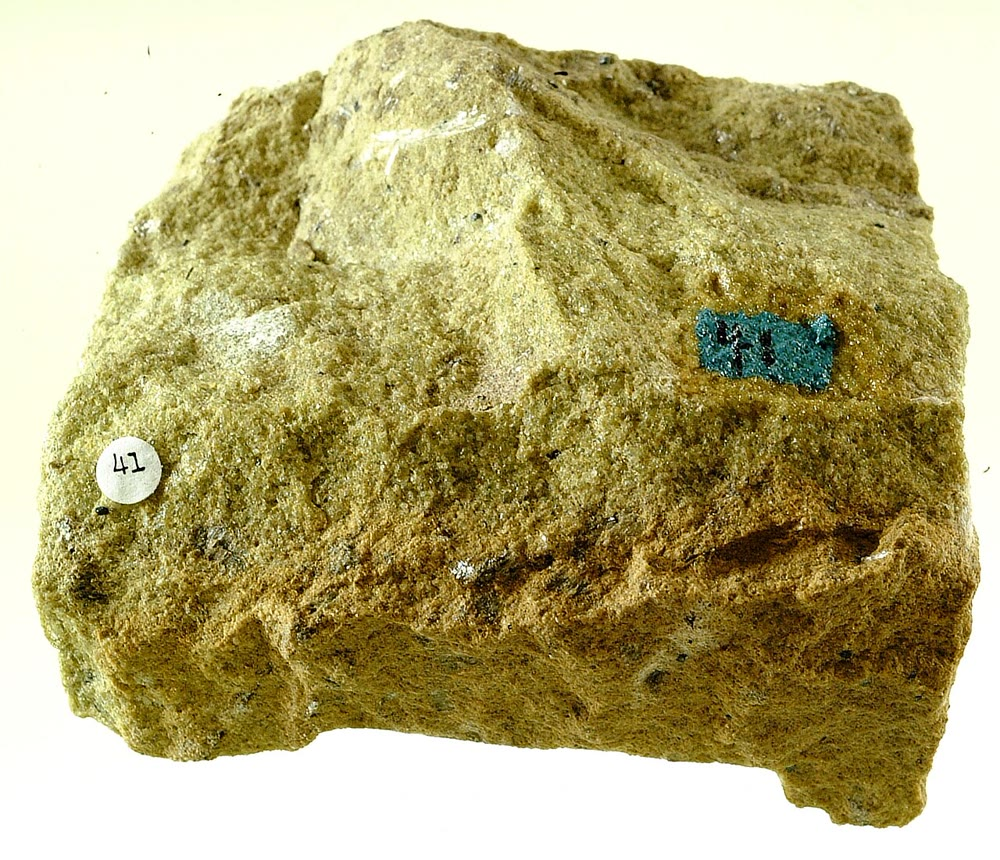
\includegraphics[width=\linewidth]{images/book4/b2-dunite.jpg}
\par\smallskip{\scriptsize \omterm{def:b2:mantle-melting:peridotites}{Dunit}, hampir seluruhnya olivin, dengan butiran hitam kecil
kromit; lebar cuplikan \qty{8.5}{cm} (Mike Davis, CC0).}
\end{minipage}
\end{inthefield}
% ledger: casetta23:kimberlite, tulane:ocean-basins (Book 2), bgs:ultramafic

\section{Latihan}

\begin{exercise}[$\star$]\label{exo:b2:mantle-melting:1}
Namailah setiap batuan dari proporsi olivin, ortopiroksen, dan klinopiroksennya
(persen): (a) 93, 5, 2; (b) 75, 25, 0; (c) 60, 27, 13; (d) 30, 45, 25. (e) Berikan
nama model mantel atas (57, 28, 13, dan spinel \qty{2}{\percent}) setelah
ketiga silikatnya dinormalkan ulang menjadi \qty{100}{\percent}.
\end{exercise}
% ledger: bgs:ultramafic, liang21:dmm-mode

\begin{exercise}[$\star$]\label{exo:b2:mantle-melting:2}
Pada diagram diopsid--anortit, cairan dengan \qty{60}{\percent} anortit
mendingin. (a) Pada suhu berapa cairan itu mulai mengkristal, dan mineral apa yang
terbentuk? (b) Pada suhu berapa mineral kedua muncul, dan bagaimana komposisi
cairan saat itu? (c) Bagaimana komposisi cairan pertama ketika
batuan dengan \qty{80}{\percent} diopsid dan \qty{20}{\percent} anortit dipanaskan,
dan pada suhu berapa cairan itu muncul?
\end{exercise}
% ledger: bowen15:di-an

\begin{exercise}[$\star$]\label{exo:b2:mantle-melting:3}
(a) Hitunglah gradien adiabatik $\alpha T/(\rho c_p)$ dalam kelvin per gigapascal
untuk $T_p = \qty{1350}{\celsius}$, $\alpha = \qty{4.0e-5}{K^{-1}}$, $\rho =
\qty{3300}{kg/m^3}$, $c_p = \qty{1000}{J/(kg.K)}$. (b) Berapa kilometer
mantel yang setara dengan satu gigapascal ($g = \qty{9.81}{m/s^2}$)? Ubahlah gradien itu menjadi kelvin
per kilometer dan bandingkan dengan gradien geotermal khas di dekat permukaan,
sekitar \qty{30}{K/km}.
\end{exercise}
% ledger: katz03:thermo, earle:settings (Book 2)

\begin{exercise}[$\star$]\label{exo:b2:mantle-melting:4}
(a) Hitunglah solidus kering \omterm{def:b2:mantle-melting:peridotites}{peridotit} pada 0, 1, 2, dan \qty{3}{GPa}. (b) Berapa
derajat solidus itu naik per gigapascal di dekat \qty{2}{GPa}? (c) Jelaskan dalam satu
kalimat mengapa mantel bersuhu \qty{1400}{\celsius} pada \qty{3}{GPa} padat, sedangkan
mantel yang sama, bila dibawa ke \qty{2}{GPa} tanpa bertukar kalor, meleleh sebagian.
\end{exercise}
% ledger: katz03:solidus

\begin{exercise}[$\star\star$]\label{exo:b2:mantle-melting:5}
Cairan dengan \qty{70}{\percent} diopsid dan \qty{30}{\percent} anortit mendingin.
(a) Taksirlah suhu likuidusnya dengan interpolasi antara likuidus pada
\qty{20}{\percent} anortit (\qty{1350}{\celsius}) dan pada \qty{40}{\percent}
(\qty{1277.5}{\celsius}). (b) Mineral mana yang mengkristal pertama? (c) Berapa fraksi massa
sistem yang telah mengkristal ketika cairan mencapai eutektik?
(d) Berapa proporsi diopsid dan anortit dalam batuan akhirnya?
\end{exercise}
% ledger: bowen15:di-an

\begin{exercise}[$\star\star$]\label{exo:b2:mantle-melting:6}
(a) Hitunglah persentase massa \ce{SiO2} dalam forsterit \ce{Mg2SiO4} dan dalam
enstatit \ce{MgSiO3} ($M_{\ce{MgO}} = \qty{40.30}{g/mol}$, $M_{\ce{SiO2}} =
\qty{60.08}{g/mol}$). (b) Bowen dan Andersen mendapati bahwa cairan peritektik terdiri atas
\qty{97.5}{\percent} \ce{MgSiO3} dan \qty{2.5}{\percent} \ce{SiO2}: berapa kadar
silikanya? (c) Gunakan aturan tuas untuk menghitung fraksi massa forsterit yang
terbentuk ketika enstatit meleleh pada peritektik, dan bandingkan dengan
\qty{5.5}{\percent} hasil mereka. (d) Apa artinya hal ini bagi kadar silika lelehan
\omterm{def:b2:mantle-melting:peridotites}{peridotit} dibandingkan dengan kadar silika ortopiroksennya?
\end{exercise}
% ledger: bowen14:mgo-sio2

\begin{exercise}[$\star\star$]\label{exo:b2:mantle-melting:7}
Dengan adiabat $T = T_p + 20P$ dan solidus kering dalam teks, hitunglah
tekanan dan kedalaman ($\qty{30.9}{km}$ per gigapascal) tempat pelelehan dimulai
untuk (a) $T_p = \qty{1300}{\celsius}$ dan (b) $T_p = \qty{1450}{\celsius}$. (c) Berapa
kilometer per \qty{10}{\celsius} awal pelelehan bertambah dalam di dekat
$T_p = \qty{1300}{\celsius}$? Gunakan \cref{prop:b2:mantle-melting:onset}.
\end{exercise}
% ledger: katz03:solidus

\begin{exercise}[$\star\star$]\label{exo:b2:mantle-melting:8}
Pada \qty{2.0}{GPa}, anggaplah \omterm{def:b2:mantle-melting:fraction}{fraksi lelehan} naik secara linear dari solidus kering sampai
likuidus \omterm{def:b2:mantle-melting:peridotites}{lherzolit} $T_{\mathrm l} = 1475.0 + 80.0P - 3.2P^2$. Untuk $F = 0.10$:
(a) hitunglah suhu batuan yang meleleh; (b) hitunglah $(\partial
T/\partial P)_F$ dan $(\partial T/\partial F)_P$; (c) hitunglah produktivitasnya dengan
$c_p = \qty{1000}{J/(kg.K)}$, $\alpha/\rho = \qty{1.21e-8}{m^3/(kg.K)}$, dan
$\Delta S = \qty{300}{J/(kg.K)}$. (d) Berapa nilainya seandainya tidak ada kalor laten?
\end{exercise}
% ledger: katz03:solidus, katz03:melting, katz03:thermo

\begin{exercise}[$\star\star$]\label{exo:b2:mantle-melting:9}
(a) Seberapa besar 1, 5, dan \qty{13}{\percent} air yang terlarut dalam lelehan menurunkan
solidus? (b) Berapa solidus jenuh air pada \qty{1}{GPa}? (c) Sebuah mantel
mengandung \qty{125}{ppm} air menurut massa, dan koefisien partisi air antara
mineral dan lelehan adalah 0.01. Pada saat pelelehan paling awal, lelehan mengandung $X =
X_{\text{total}}/D$: hitunglah nilai itu dan penurunan solidus yang ditimbulkannya.
\end{exercise}
% ledger: katz03:water

\begin{exercise}[$\star\star\star$]\label{exo:b2:mantle-melting:10}
(a) Pada \cref{prop:b2:mantle-melting:triangle}, periksalah bahwa mantel yang memasuki
dasar segitiga setiap tahun sama dengan mantel yang keluar melintasi sisi-sisinya. Mengapa
sisi-sisinya harus miring \ang{45} untuk mantel yang naik dengan kecepatan $U$ dan keluar dengan kecepatan $U$?
(b) Tunjukkan bahwa, dengan produktivitas tetap $\Pi$ per gigapascal, $h_c = \Pi\,\rho
g\,z_0^2/2$ (dengan $P_0 = \rho g z_0$), sehingga kerak bertambah sebanding dengan kuadrat
kedalaman awal pelelehan. (c) Sebuah punggungan memekar dengan laju penuh \qty{50}{mm/yr} dan
menghasilkan kerak setebal \qty{7.1}{km}: berapa volume kerak yang dihasilkan setiap kilometer punggungan
per tahun, dan berapa volume mantel yang dilelehkannya jika \omterm{def:b2:mantle-melting:fraction}{fraksi lelehan} rata-ratanya
\qty{12}{\percent}?
\end{exercise}

\begin{exercise}[$\star\star\star$]\label{exo:b2:mantle-melting:11}
Dalam sistem terner pada gambar skematis, cairan $X$ mengandung
\qty{60}{\percent} A, \qty{20}{\percent} B, dan \qty{20}{\percent} C;
eutektik biner $e_{AB}$ terletak pada A 40, B 60 (persen), dan \omterm{def:b2:mantle-melting:ternary}{eutektik terner} E pada
A 25, B 30, C 45. (a) Tuliskan komposisi cairan ketika fraksi massa $t$
A murni telah mengkristal, dan tunjukkan bahwa rasio B terhadap C tetap 1. (b) Kotektik
dari $e_{AB}$ ke E adalah garis titik-titik $e_{AB} + s(E - e_{AB})$: tentukan
tempat cairan bertemu dengannya, dan fraksi A yang telah mengkristal saat itu. (c) Ketika
cairan mencapai E, berapa fraksi sistem yang masih cair? (C tidak masuk ke kristal
mana pun sebelum E.) (d) Berapa banyak A dan berapa banyak B yang telah mengkristal saat itu?
\end{exercise}

\begin{exercise}[$\star\star\star$]\label{exo:b2:mantle-melting:12}
Kadar air lelehan jenuh adalah $X_{\mathrm{sat}} = 12P^{0.6} + P$
(persen, $P$ dalam gigapascal). (a) Hitunglah nilainya pada 1 dan \qty{2}{GPa}, penurunan solidus
yang ditimbulkannya, dan solidus jenuh air pada kedua tekanan. (b) Mengapa
solidus jenuh hampir tidak berubah antara 1 dan \qty{2}{GPa}, sedangkan solidus kering
naik lebih dari \qty{100}{\celsius}? (c) Di dalam baji mantel pada \qty{2}{GPa} dan
\qty{1100}{\celsius}, berapa banyak air yang harus dikandung lelehan agar batuan meleleh?
\end{exercise}
% ledger: katz03:water, katz03:solidus

\section{Soal: Di bawah punggungan}

\begin{problem}[{Soal akhir pekan --- dari adiabat mantel ke tebal
kerak samudra, lalu kembali ke suhu mantel}]
\label{pb:b2:mantle-melting:1}
Mantel naik di bawah punggungan menyusuri adiabat dan meleleh. Data: koefisien
muai termal $\alpha = \qty{4.0e-5}{K^{-1}}$; massa jenis $\rho = \qty{3300}{kg/m^3}$;
kalor jenis $c_p = \qty{1000}{J/(kg.K)}$; entropi pelelehan $\Delta S =
\qty{300}{J/(kg.K)}$; $g = \qty{9.81}{m/s^2}$; solidus kering $T_{\mathrm s} =
1085.7 + 132.9P - 5.1P^2$ dan likuidus \omterm{def:b2:mantle-melting:peridotites}{lherzolit} $T_{\mathrm l} = 1475.0 +
80.0P - 3.2P^2$ (\unit{\celsius}, $P$ dalam \unit{GPa}); produktivitas rata-rata model
pelelehan hasil pencocokan, $\Pi = \qty{9}{\percent}$ per gigapascal; koefisien reaksi
klinopiroksen di dekat permukaan 0.50; kerak teramati \qty[uncertainty-mode=separate]{7.1 \pm 0.8}{km}
di punggungan normal dan \qty{20}{km} di atas inti plume Islandia. Anggaplah mantel
dan kerak bermassa jenis sama.

\noindent\textbf{Bagian I --- Tempat pelelehan dimulai.}
\begin{enumerate}
\item Ubahlah $T_p = \qty{1350}{\celsius}$ menjadi kelvin.
\item Hitunglah gradien adiabatik $\alpha T_p/(\rho c_p)$ dalam kelvin per
gigapascal, dan bulatkan ke puluhan terdekat.
\item Berapa kilometer mantel yang setara dengan satu gigapascal? Nyatakan gradien itu dalam
kelvin per kilometer.
\item Dengan adiabat $T = 1350 + 20P$, tuliskan persamaan kuadrat untuk tekanan awal pelelehan
$P_0$ dan selesaikan.
\item Berikan kedalaman dan suhu tempat pelelehan dimulai.
\item Periksalah bahwa solidus pada $P_0$ memberikan suhu yang sama.
\end{enumerate}

\noindent\textbf{Bagian II --- Berapa banyak lelehan.}
\begin{enumerate}[resume]
\item Pada \qty{1.5}{GPa}, hitunglah solidus, likuidus \omterm{def:b2:mantle-melting:peridotites}{lherzolit}, dan
selisih keduanya.
\item Dengan \omterm{def:b2:mantle-melting:fraction}{fraksi lelehan} yang naik secara linear di antara keduanya, berikan suhu
batuan pada $F = 0.10$, dalam derajat Celsius dan dalam kelvin.
\item Hitunglah $(\partial T/\partial P)_F$ dan $(\partial T/\partial F)_P$ di sana.
\item Hitunglah produktivitas menurut \cref{prop:b2:mantle-melting:productivity}, dalam
persen per gigapascal.
\item Model hasil pencocokan memberikan rata-rata $\Pi = \qty{9}{\percent}$ per gigapascal.
Mengapa lebih rendah? Dengan $\Pi$, berapa \omterm{def:b2:mantle-melting:fraction}{fraksi lelehan} $F_{\max}$ yang tercapai di
permukaan?
\item Model mantel itu mengandung klinopiroksen \qty{13}{\percent}. Pada \omterm{def:b2:mantle-melting:fraction}{fraksi lelehan}
berapa klinopiroksen itu habis di dekat permukaan? Apakah residu di bawah sumbu berupa
\omterm{def:b2:mantle-melting:peridotites}{lherzolit} atau \omterm{def:b2:mantle-melting:peridotites}{harzburgit}?
\end{enumerate}

\noindent\textbf{Bagian III --- Kerak.}
\begin{enumerate}[resume]
\item Gunakan \cref{prop:b2:mantle-melting:triangle} dengan $H = z_0$ untuk menghitung
tebal kerak.
\item Berapa \omterm{def:b2:mantle-melting:fraction}{fraksi lelehan} rata-rata lelehan gabungan?
\item Bandingkan dengan tebal yang teramati.
\item Model lengkap pada gambar memberikan \qty{9.0}{km}. Mengapa lebih tipis daripada
taksiranmu?
\item Tunjukkan bahwa $h_c = k P_0^2$ dan hitunglah $k$ dalam kilometer per
gigapascal kuadrat.
\end{enumerate}

\noindent\textbf{Bagian IV --- Suhu mantel.}
\begin{enumerate}[resume]
\item Hitunglah tekanan awal pelelehan $P_0$ yang menghasilkan kerak setebal \qty{7.1}{km}.
\item Berikan kedalaman awal pelelehan yang bersesuaian.
\item Dengan adiabat $T = T_p + 20P$, hitunglah suhu potensial yang
menempatkan awal pelelehan pada tekanan itu.
\item Ulangi perhitungan untuk 6.3 dan \qty{7.9}{km}: rentang $T_p$ berapa yang
diizinkan oleh sebaran tebal kerak?
\item Kerak setebal \qty{20}{km} di atas inti plume Islandia. Hitunglah
suhu potensial di sana, dan kelebihannya terhadap suhu potensial pada pertanyaan~20.
\item Lava pulau samudra menunjukkan plume yang 200 sampai \qty{300}{\celsius} lebih panas daripada
mantel di sekitarnya. Kemukakan mengapa kerak memberikan kelebihan yang lebih kecil.
\item Berapa persen kerak menebal untuk mantel yang \qty{10}{\celsius}
lebih panas, di dekat punggungan normal?
\item Punggungan yang sangat lambat menghasilkan kerak yang lebih tipis. Jelaskan alasannya dengan segitiga itu.
\item Nyatakan \omterm{def:b2:mantle-melting:tp}{suhu potensial mantel} di bawah punggungan normal yang
diberikan oleh tebal kerak, yaitu angka kunci soal ini, dan bandingkan
dengan \qty{1350}{\celsius} dari fisika mineral dan rentang 1280 sampai
\qty{1400}{\celsius} dari lava.
\end{enumerate}
\end{problem}
% ledger: katz03:solidus, katz03:melting, katz03:thermo, white:crust (Book 3), herzberg:tp (Book 3), katsura:adiabat (Book 3)
